\section{Evaluation protocol}
\label{sec:evaluation}

\subsection{Questions and evidence layers}

E1--E3 provide controlled implementation evidence through constructed histories, scripted review interactions, and fixed workloads. E1 tests why exact candidate binding matters when values and retained context agree. E2 locates the review-to-confirmation boundary of that guarantee. E3 measures the costs of enforcement and querying.

\begin{description}[leftmargin=2.6em,labelwidth=2.1em]
\item[RQ1] Do the formal and concrete checks support the admission contract, and what changes when a rich event journal records the exact reviewed candidate?
\item[RQ2] Which inconsistencies between recorded review intent and confirmation can server-held session binding reject, and which remain outside its guarantee?
\item[RQ3] What admission, reverse-trace, and storage costs occur on the repaired implementation under the declared workloads?
\end{description}

E1--E3 use the equality-repaired reference at commit \code{c6d512843c905cab6d8521dd8c914f7fb26d85ae}, after rerunning implementation regressions and harness checks. The earlier Alloy, projection, and catalogue results remain separate evidence. The prospective local protocol, pilot amendments, environment, raw receipts, and execution status are documented in Online Resource 1, Sections S1 and S6. E1--E3 make no hosted-model calls; historical agent runs remain separate in S5.

Execution, query-answer, browser-case, and timing counts have separate denominators.

\Cref{fig:evidence-route} summarizes the evidence route from the admission relation to E1--E3.

\begin{figure}[htbp]
\centering
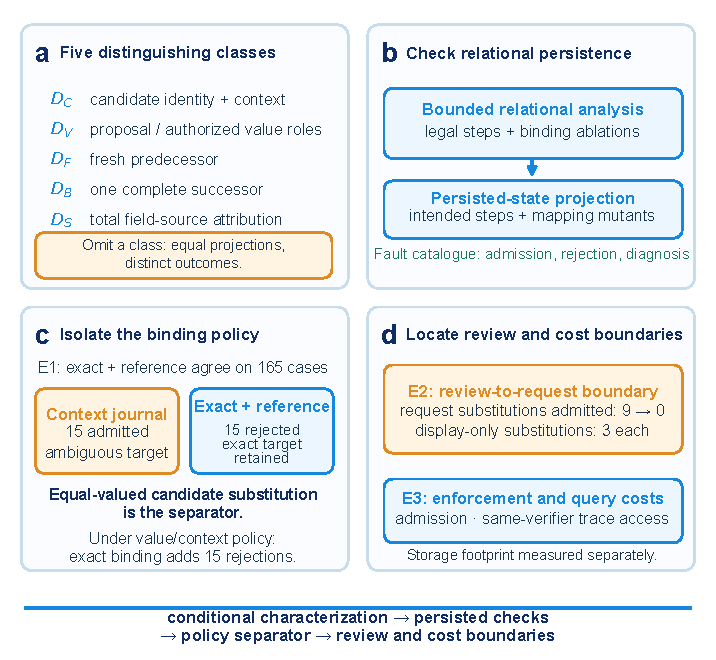
\includegraphics[width=0.975\textwidth]{Fig2.pdf}
\caption{Evidence route from the conditional characterization to persistence checks and E1--E3. E1 supplies the policy separator; E2 tests request binding and the presentation boundary; E3 characterizes enforcement and query costs. Displayed E1/E2 results are read from archived tables; timing totals are checked against CSV summaries. Diagram scripting assisted by OpenAI Codex}
\label{fig:evidence-route}
\end{figure}

\subsection{RQ1: rich-context and exact-binding comparison}

A separately written \code{sqlite3} journal retains immutable candidates/events, review context, versions, transactions, and complete field sources. Its \emph{context} configuration checks field, version, evidence, and retained context while omitting candidate/certificate identifiers and instance-creation time. Its \emph{exact} configuration adds the reviewed-candidate link. The third arm invokes the reference's actual transaction. We score both instance authorization and the looser value/context policy.

Fifteen inputs cross eleven case families and three mechanisms. Twelve deterministically selected archived proposal cells contain four distinct values; three synthetic type controls bring the total to seven. They enter newly constructed histories, rather than complete historical-task replays. Cases exercise Accept, Correction, multi-field admission, equal-valued candidate and different-evidence substitutions, staleness, replay, unauthorized value, and three interrupted transaction locations. Online Resource 1, Section S6 lists the inputs and cases.

After acceptance, an independent reader checks six provenance questions on three fields: proposal, authorized value, reviewer, reviewed candidate, current value, and source version. Each accepted history contributes eighteen answers, classified as correct, wrong, ambiguous, or unavailable. Rejection requires the expected reason and unchanged logical fact-database digest, measured after authorization preparation. Prior review records may persist. Original strengthened-baseline continuity checks have a separate denominator.

\subsection{RQ2: review-to-confirmation boundary}

Local Chrome/Playwright runs an instrumented review fixture backed by \code{ReviewForms.confirm}. An independent driver records the displayed candidate, proposal, and authorized value before confirmation. Three JSON inputs cross ten interactions and two paths, giving sixty cases; six confirmations separately prepare replay setups. Positive controls cover acceptance, correction, and reselection. Candidate/value/principal request substitutions, stale/replayed requests, interrupted commits, and display-only substitution probe distinct boundaries.

The original path is compared with a server-held session binding candidate, version, reviewer, and value. Acceptance, agreement with recorded review intent, and writes on rejection are recorded. The fixture uses fixed principal labels and a separate session database. The resulting request and presentation boundaries are interpreted in \cref{sec:discussion}.

\subsection{RQ3: current-version costs}

Two ten-cell admission comparisons contribute 4,000 observations each; a 36-cell trace comparison contributes 14,400. Each cell has five warmups and 200 timed calls per arm in seeded randomized order, for 22,400 timed observations excluding warmups. Environment versions and full grids are in Online Resource 1, Sections S1, S4, and S6.

The mechanism comparison times complete confirmation on shared recognition-source workloads. Construction and database cloning are excluded: the journal opens its connection before timing, whereas the reference may connect lazily inside confirmation. The study measures these complete call boundaries; \cref{sec:discussion} explains their implementation differences.

A separate manual-source materialization ablation times persistence of a prevalidated delta while retaining authority rows, complete sources, transactionality, and CAS. Its result must match the precomputed relational fingerprint. Validation and planning occur outside that timer; its full-path column belongs to a different workload from the mechanism comparison.

The trace comparison holds the verifier fixed and changes three bulk repository reads to identifier enumeration and point lookups. Every returned complete object must agree. The grid varies record width, history length, and total records. Storage fixtures populate full/reduced schemas at three transition scales; their footprint excludes external evidence/model outputs, and the reduced schema has fewer audit obligations.
